\section{Overview}
\label{sec: overview}%
In this section, a general description of the architecture of the \verb|CKB| system is provided.
The main aspects of the design are:
\begin{itemize}
    \item \textbf{Client-Server architecture. } It consists of a presentation tier, an application and a data tier.
    The firsts one allow the user to communicate with the server and shows him through the UI the answers it receives back from the application tier.
    The second one receives requests from users, elaborates answers, changes the status communicating with the data tier and sends back the needed information to users.
    Finally, the data tier stores, updates, and handles the information.
    \item \textbf{Microservices. } Functionalities of the system are divided into several services in order to reduce dependencies between
    modules and to increase scalability, availability and maintainability of the system.
\end{itemize}

\section{Component View}
\label{sec: component_view}%
The component diagram shows all the identified components.
It also describes the relations between the modules, representing the verse of the communication flow and the actors participating.

Bla bla bla

\subsection{Component diagram}
\label{subsec:component_diagram}%
\begin{figure} [H]
    \begin{center}
        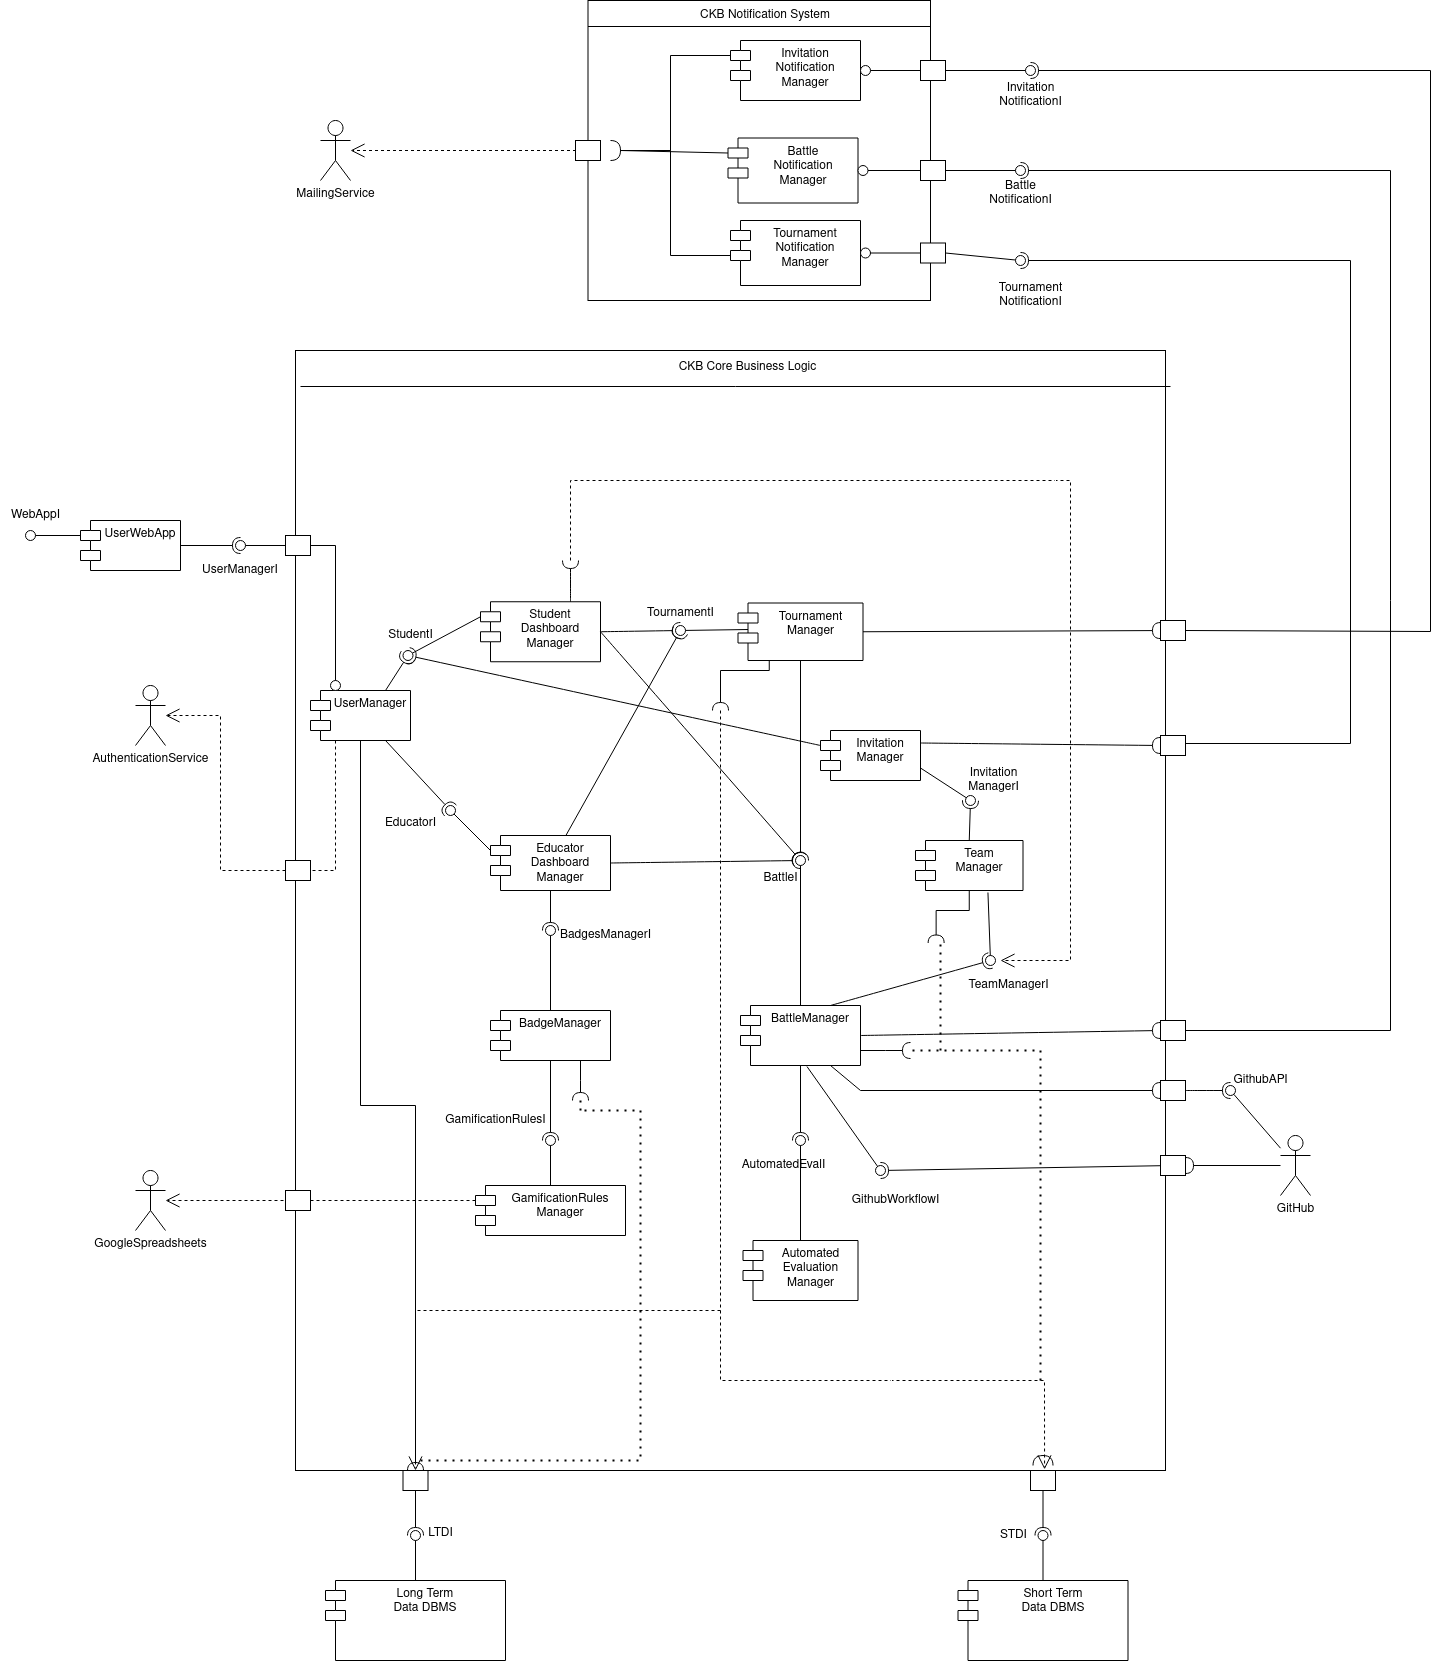
\includegraphics[width=1\linewidth]{Images/compdiag.png}
        \caption{Component diagram of the CKB platform.}
        \label{fig: cd}
    \end{center}
\end{figure}

\subsection{Components description}
\label{subsec:components_description}%
The components are:
\begin{itemize}
    \item \textbf{User WebApp.} \verb|User| \verb|WebApp| is the front-end for users. 
    %It allows them to interact with the system by offering the following functions through the interface UserAppI:
    %    \begin{itemize}
    %        \item \textbf{Register} 
    %        \item \textbf{Login} 
    %        \item \textbf{A} 
    %        \item \textbf{Z} 
    %        \item \textbf{Z} 
    %        \item \textbf{Z} 
    %        \item \textbf{Z} 
    %        \item \textbf{Z} 
    %    \end{itemize}
    \item \textbf{UserManager} \verb|UserManager| component offers, through the interface \verb|UserManagerI|, the basic function for handling users:
        \begin{itemize}
            \item \textbf{Register}
            \item \textbf{Login}
            %tanta altra roba di sicuro
        \end{itemize}
        It also provides user information to the \verb|EducatorDashboardManager| component and the \verb|StudentDashboardManager| component depending on the role of the logged user.
    %EducatorDashboardManager
    \item \textbf{Educator Dashboard Manager.} \verb|Educator| \verb|Dashboard| \verb|Manager| handles the main functionalities accessible by an Educator. 
    It allows creating and managing both CodeKataBattles and Tournaments, defining new badges and rules and performing all the operations that an Educator should be able to perform according to the RASD.
    \item \textbf{Badge Manager.} \verb|Badge| \verb|Manager| is used to manage badges, allowing to perform operations such as assigning a badge to a Student, creating new badges and defining new rules and variables to obtain them.
    \item \textbf{Gamification Rules Manager.} \verb|Gamification| \verb|Rules| \verb|Manager| is used to manage rules and variables used to determine winners of badges. 
    This component relies on an external actor, Google Spreadsheet, to allow defining new rules in a simple but effective way (Spreadsheet formulas).
    \item \textbf{Student Dashboard Manager.} \verb|Student| \verb|Dashboard| \verb|Manager| handles the main functionalities accessible by a Student.
    It allows joining and participating in CodeKataBattles and Tournaments, checking the status of the ongoing ones and the results of the past ones.
    \item \textbf{Battle Manager.} \verb|Battle| \verb|Manager| is used to manage CodeKataBattles, allowing to perform operations such as creating a new CodeKataBattle, 
    joining an existing one and checking the status of the ongoing ones through its interface \verb|BattleI|.
    \item \textbf{Tournament Manager.} \verb|Tournament| \verb|Manager| is used to manage Tournaments, allowing to perform operations such as creating a new Tournament,
    joining an existing one and checking the status of the ongoing ones through its interface \verb|TournamentI|. Educators can also add other Educators as admin to a tournament they created.
    \item \textbf{Automated Evaluation Manager.} \verb|Automated| \verb|Evaluation| \verb|Manager| is used to manage the automated evaluation of CodeKataBattles assigning scores to teams.
    \item \textbf{Team Manager.} \verb|Team| \verb|Manager| is used to manage teams, allowing to perform operations such as creating a new team, joining an existing one and inviting a student to join a team.
    %invitations manager
    \item \textbf{Notification Manager.} \verb|Notification| \verb|Manager| allows Students to be notified via email when a new CodeKataBattle or Tournament is created or ends. It relies on an external Mailing Service.
\end{itemize}
External entities are:
\begin{itemize}
    \item \textbf{Google Spreadsheet.} \verb|Google| \verb|Spreadsheets| is the engine used by Educators when creating new rules for badges. 
    \item \textbf{Mailing Service.} \verb|Mailing| \verb|Service| is used to send emails to Students when a new CodeKataBattle or Tournament is created or ends.
    \item \textbf{Github.} \verb|Github| interacts with the \verb|Battle| \verb|Manager| component to handle the code that represents the solution of a CodeKataBattle. 
    CKB platform offers APIs to allow Github Actions Workflow to trigger a pull request to the repository of the solution.
\end{itemize}

\section{Deployment View}
\label{sec: deployment_view}%
The distribution of components capturing the topology of the system is illustrated below by using a deployment diagram.
The system is structured in a multitier architecture.
\newline
\begin{figure} [H]
    \begin{center}
        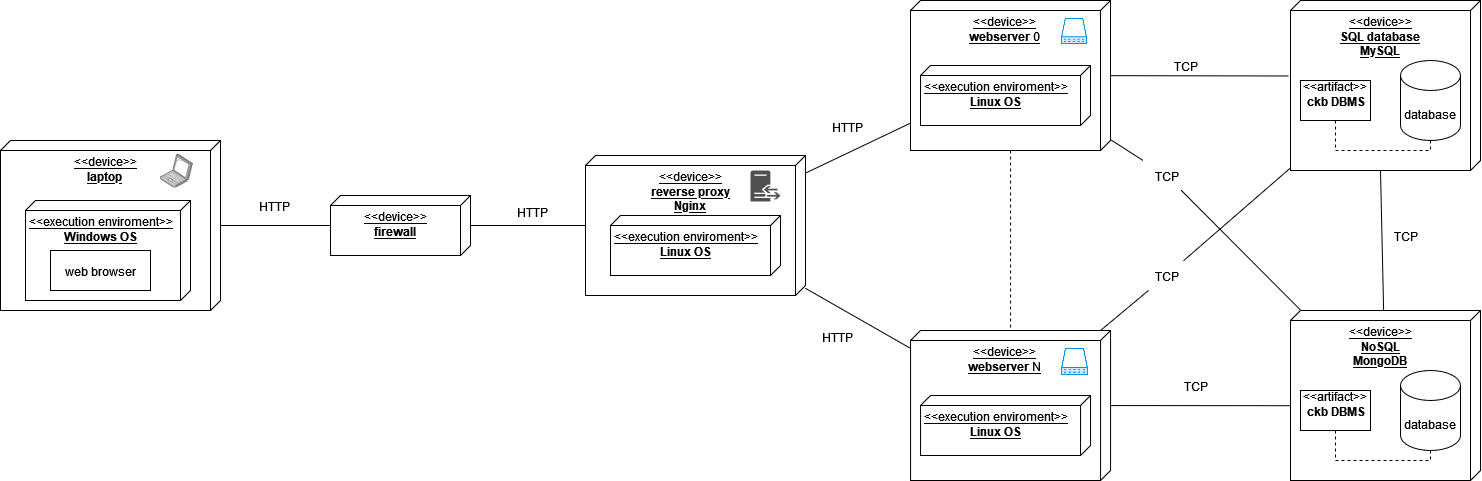
\includegraphics[width=1\linewidth]{Images/deployment_diag.png}
        \caption{Deployment diagram of the CKB platform.}
        \label{fig: depl_diagram}
    \end{center}
\end{figure}


\noindent\textbf{Laptop devices}\newline
This node represents a user's laptop, which is the client-side hardware. The "Windows OS" indicates that the laptop is running on the Windows operating system. 
The "web browser" is the software application used to access the web interface of the platform.

\noindent\textbf{Firewall}\newline
This is a security device that monitors and filters incoming and outgoing network traffic based on an organization's previously established security policies. 
Here, it acts as a barrier between secure internal networks and untrusted external networks, such as the internet.

\noindent\textbf{Reverse Proxy}\newline
This server is running Nginx, which is a web server that can also be used as a reverse proxy. This means it can distribute traffic to various servers, 
thereby acting as an additional layer of abstraction and control to smooth the flow of network traffic between clients and services.

\noindent\textbf{Webserver 0}\newline
This is one of potentially multiple web servers that handle the incoming HTTP requests from the client's web browser, process those requests, 
and serve the appropriate web pages. It runs on a Linux operating system, which suggests a preference for open-source solutions.

\noindent\textbf{Webserver N}\newline
This indicates there are multiple webservers in this deployment, following a similar configuration to "Webserver 0." 
The "N" represents an indefinite number, showing that the architecture is scalable and can include as many webservers as needed.

\noindent\textbf{SQL database (MySQL)}\newline
This database node uses MySQL, which is a relational database management system (RDBMS) based on SQL (Structured Query Language). 
It's used to store and manage the platform's structured data efficiently.

\noindent\textbf{NoSQL database (MongoDB)}\newline
This is a NoSQL database, specifically MongoDB, which is designed for storing unstructured data. It offers high performance, high availability, and easy scalability.

\noindent\textbf{ckb DBMS}\newline
This artifact within both database nodes represents the database management software that's part of the CodeKataBattle platform. It is likely the collection of schemas, 
tables, queries, reports, views, and other objects associated with the platform's database management.

\section{Selected architectural styles and patterns}

In this section are shown the most relevant architectural design choices, with also the explanation of their role and their advantages.

\textbf{3 Tier Architecture}\newline
N-tier architecture refers to the structure of a software application divided into multiple tiers. 
A tier is a layer of the application that operates on its own infrastructure or server. 
In particular, we decided to implement a 3-tier architecture. The tiers are: presentation, logic, and data tier.\newline
Presentation tier → It presents information to users and receive user inputs\newline
Logic tier → It handles business logic and application processing logic. It’s responsible for processing user requests, 
applying business rules, and managing the flow of data between the presentation and data tier\newline
Data tier → It manages the storing and retrieving of the data. It handles data persistence and integrity too\newline
The advantages of using this type of architecture revolve around its scalability, ease of management, and flexibility and security. 
If we need to add more resources to a specific tier or modify it, we can do so without affecting the other tiers. Moreover, we can secure each 
of the three tiers separately using different methods and techniques, based on the security needed for the specific tier

\textbf{WebSocket with Pub/Sub Pattern}\newline
The WebSocket protocol provides a full-duplex communication channel over a single TCP connection. 
This means that data can be sent and received at the same time, allowing for real-time communication between the client and the server.
The Publish/Subscribe pattern is a messaging pattern where senders (publishers) categorize messages into classes without knowing which 
subscribers (if any) there might be. Similarly, subscribers express interest in one or more classes, and only receive messages that are of interest, 
without knowing which publishers there are
When combined, WebSocket and Pub/Sub can be a powerful tool for real-time web applications. Regarding the CKB specifically:\newline
1. Publishing → when an event occurs in CKB (e.g., a new battle is created, a score is updated,…), the server publishes a message about this event. 
The message is categorized based on the type of event (e.g., “New Battle”, “Score Updated”,…)\newline
2. Subscribing → Clients (users of CKB) subscribe to the types of events they’re interested in. 
For example, a student might subscribe to “New Battle” events to be notified when a new battle is created.\newline
3. Real-Time Updates → Because the communication is happening over WebSocket, these messages can be pushed from the 
server to the client in real-time. As soon as a new message is published, all clients subscribed to that type of event will receive the message.\newline
4. Scalability → The Pub/Sub pattern allows for scalability. As the number of users (subscribers) and events (publishers) increases, 
the system can continue to function efficiently.\newline
This combination of WebSocket and Pub/Sub can provide a dynamic, real-time user experience for CKB, making it more engaging and responsive for its users.

\textbf{Worker Pooling}\newline
Worker pooling refers to a pattern where a set of initialized “workers” (threads, processes, or any kind of parallel-executing entities) 
are kept ready to perform a certain kind of task. In the context of CKB, worker pooling can help to improve the performance and 
responsiveness of your server by reusing workers instead of creating new ones for each request. This can be particularly helpful in 
a high-load scenario where new requests are coming in faster than the server can create new workers. 
Moreover, thanks to the presence of the reverse proxy, we can obtain a balanced load cross the network. 
Infact, a reverse proxy can distribute incoming requests to multiple server replicas. 
This is done to achieve evenly distributed load across the servers replica, 
preventing any single server from becoming a bottleneck. 
Each replica would have its own worker pool to handle the requests it receives

\textbf{Microservices}\newline
The application uses a suite of small services, instead of being monolithic, 
each running in its own process and communicating with the other microservices. 
To communicate between each other, microservices can exploit an event-driven paradigm (like publisher and subscriber). 
Moreover, other design choice must be taken into consideration, for example to achieve resiliency. 
One suggestion could be to utilize a Circuit Breaker to inhibit all those microservices that are failing repeatedly. 
In the specific context of CKB, this could be momentarily debilitating some functions of the platform, 
such as the possibility to visualize the leaderboard of a Tournament or adding members to a team. 
This way, the platform itself can keep running, and maintenance can be executed on the faulty microservices to bring them back up as quickly as possible

\textbf{Database: NoSQL with SQL}\newline
In the context of CodeKataBattle (CKB), the use of two different databases, MongoDB (a NoSQL database) and MySQL (a SQL database), 
is a strategic decision aimed at leveraging the strengths of both types of databases to efficiently manage and access data.

MongoDB, a document-oriented database, offers flexibility with its schema-less design, 
making it suitable for storing diverse data types like users, educators, tournament results, badges, notifications, etc. 
This flexibility allows for easy and quick modifications as the data requirements evolve over time.

On the other hand, MySQL, a relational database, 
excels in handling structured data and complex queries. 
It’s used for storing tournaments, teams, and battles, which are likely to involve numerous queries, 
especially during an ongoing tournament. The structured nature of SQL databases allows for efficient querying and retrieval of data, 
ensuring smooth operation during high-load scenarios.

The entity ‘Tournament’ is shared between both databases, 
necessitating synchronization to ensure data consistency. 
This dual-database approach combines the flexibility of MongoDB with the query efficiency of MySQL, 
providing a robust and adaptable data management solution for CKB.

\section{Other Design decisions}

\textbf{Firewall}\newline
A firewall is a network security system that monitors and controls incoming and outgoing traffic based on predetermined security rules. 
The firewall sits between the CKB’s network and the larger internet, examining all network traffic and blocking any 
that doesn’t meet its configured security rules. This can help protect CKB from various types of attacks, 
such as SQL injection, cross-site scripting and other exploits that could take advantage of vulnerabilities in the web application. 
Moreover, a firewall can prevent unauthorized data from leaving the web application, adding an extra layer of data protection. 
This is particularly important for a platform like CKB, which might handle sensitive data such as coding challenge solutions and users’ info. 
The firewall must be configured to allow WebSocket traffic, which is used for real-time updates in CKB.


\textbf{Model-View-Controller (MVC)}\newline
The Model-View-Controller (MVC) is a design pattern widely used in software development, particularly in object-oriented programming and web application. 
It separates an application into three main logical components: the Model, the View, and the Controller\newline
Model → The Model contains the methods for accessing data useful to the application. 
In CKB, this could include data related to users, battles, tournaments, scores, etc. The Model directly manages the data, logic, and rules of the application\newline
View → The View is responsible for displaying data to the user and managing the interaction between the user and the underlying infrastructure. 
In CKB, this could include the user interfaces for viewing and joining battles, viewing scores, etc.\newline
Controller → The Controller receives user commends through the View and reacts by performing operations that can affect the Model and 
generally lead to a change of state in the View. In CKB, this could include operations like creating a new battle, etc.\newline
The MVC pattern simplifies the code of applications by logically separation concerns. 
This separation allows developers to focus on one aspect of the software at a time, making the code easier to understand, maintain, and expand. 
It also improves efficiency by allowing different parts of the code to be developed and tested independently.

